\section{Data Description}

\subsection{Data Source}

Bacterial proteins for the bac network 
were extracted from full bacterial sequences using Prodigal. 
Viral proteins for the vir network were extracted from viral metagenomic contigs 
after de novo assembly using Prodigal. 

Protein similarity networks were constructed using MMseqs2, a sequence comparison tool 
designed for fast and sensitive large-scale sequence alignment.
Pairwise protein similarities were computed, 
and an edge between two proteins was included in the network if their bit score 
exceeded a threshold of 50.

The resulting networks therefore represent weighted protein similarity 
graphs based on sequence homology. The data originally come from the paper:

\begin{center}
\textit{Whole-Virome Analysis Sheds Light on Viral Dark Matter in Inflammatory Bowel Disease}
\end{center}


\subsection{Descriptive Comparison of Bac and Vir}

The bac network consists of 819 nodes and 88,914 edges, while the vir network
consists of 1,603 nodes and 25,507 edges, meaning the vir network is approximately twice as large
as the bac network. However, the bac network is substantially denser.

The density of the bac network is computed as follows:

\[
\text{Density} = \frac{2E}{N(N-1)} = 
\frac{2 \cdot 88914}{819 \cdot 818} \approx 0.265
\]

meaning that 26.5\% of all possible edges are present in the bac network.

In contrast, the density of the vir network is:

\[
\text{Density} = \frac{2E}{N(N-1)} = 
\frac{2 \cdot 25507}{1603 \cdot 1602} \approx 0.0199
\]

meaning that only 1.99\% of all possible edges are present in the vir network.

The average degree of the bac network is:

\[
\text{Average Degree} = \frac{2E}{N} = \frac{2 \cdot 88914}{819} \approx 217.1
\]

while the average degree of the vir network is:

\[
\text{Average Degree} = \frac{2E}{N} = \frac{2 \cdot 25507}{1603} \approx 31.8
\]

meaning that, on average, bac proteins are approximately seven times more similar to other proteins
than vir proteins.

Based on the substantially higher average connectivity of the bacterial network, 
its degree distribution is expected to be comparatively homogeneous and 
concentrated around higher degree values. The dense connectivity suggests 
the presence of strongly interconnected subclusters, potentially approaching 
quasi-complete structures within communities.

In contrast, the viral network is expected to exhibit a more heterogeneous and 
potentially heavy-tailed degree distribution. 
Such a structure would be characterized by a small number of highly 
connected hub nodes and a large proportion of weakly connected proteins, 
reflecting a sparse and modular topology.

By computing the degree distribution of both networks,
the structural differences can be visualized using a histogram:

\begin{center}
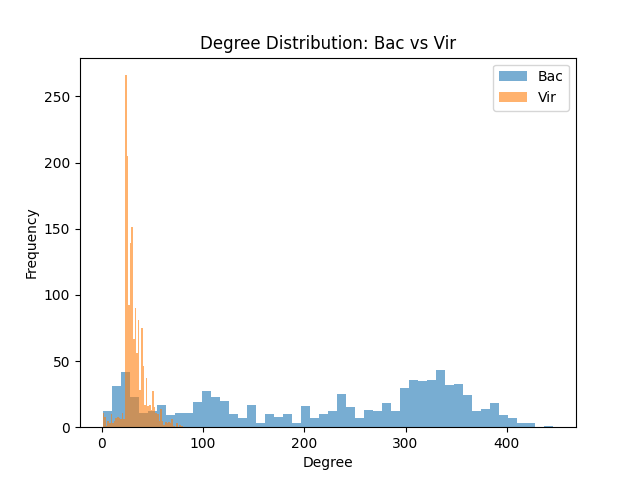
\includegraphics[width=0.8\textwidth]{Figures/data_description/data_distribution_comparison.png}
\end{center}

The histogram clearly shows that the bacterial network is characterized by 
substantially higher node degrees compared to the viral network. 
While the viral network exhibits a strong concentration of low-degree nodes, 
the bacterial network displays a broad distribution extending to very high degree values.
This indicates a much denser and more interconnected structure in the bacterial network,
whereas the viral network appears sparse and modular.

\subsection{Network Construction}

The networks are constructed based on sequence similarity between proteins.
Nodes represent proteins, and edges represent sequence similarity between them.
The weight of each edge is calculated using the bit score,
which is a normalized measure of sequence similarity derived from 
the raw alignment score.

The bit score is computed using the following formula:

\[
S' = \frac{\lambda S - \ln K}{\ln 2}
\]

where \(S\) is the raw alignment score, \(\lambda\) and \(K\) 
are statistical parameters derived from the scoring system used in the sequence alignment,
and \(\ln\) denotes the natural logarithm.

The bit score provides a standardized way to compare sequence 
similarities across different alignments, allowing for a more 
meaningful interpretation of the edge weights in the 
context of protein similarity networks.

